\documentclass{article}
\usepackage[margin=1in]{geometry}

\usepackage{microtype}
\usepackage{graphicx}
\usepackage{subfigure}
\usepackage{booktabs}
\usepackage{hyperref}
\newcommand{\theHalgorithm}{\arabic{algorithm}}

\usepackage{xcolor}
\definecolor{fluor}{RGB}{204,255,0}
\definecolor{alert}{RGB}{255,153,51}

% For theorems and such
\usepackage{amsmath}
\usepackage{amssymb}
\usepackage{mathtools}
\usepackage{amsthm}
\usepackage{bm}

%%%%%%%%%%%%%%%%%%%%%%%%%%%%%%%%
% THEOREMS
%%%%%%%%%%%%%%%%%%%%%%%%%%%%%%%%
\theoremstyle{plain}
\newtheorem{theorem}{Theorem}[section]
\newtheorem{proposition}[theorem]{Proposition}
\newtheorem{lemma}[theorem]{Lemma}
\newtheorem{corollary}[theorem]{Corollary}
\theoremstyle{definition}
\newtheorem{definition}[theorem]{Definition}
\newtheorem{assumption}[theorem]{Assumption}
\newtheorem{problem}[theorem]{Problem}
\theoremstyle{remark}
\newtheorem{remark}[theorem]{Remark}
\newtheorem{example}[theorem]{Example}
\newtheorem{ansatz}{Ansatz}

%%%%%
% Custom macros in ref.tex (keep the same copies)
%%%%%
\newcommand{\E}{\mathbb{E}}
\newcommand{\Var}{\mathrm{Var}}
\newcommand{\Cov}{\mathrm{Cov}}
\newcommand{\R}{\mathbb{R}}
\newcommand{\N}{\mathbb{N}}

\DeclareMathOperator*{\argmin}{arg\,min}
\DeclareMathOperator*{\argmax}{arg\,max}

% Vectors, matrices, sets – conventions used throughout ref.tex
% (icml2025 loads what is needed so \bm is available)
\newcommand{\vx}{\bm{x}}
\newcommand{\vg}{\bm{g}}
\newcommand{\vnu}{\bm{\nu}}
\newcommand{\vd}{\bm{d}}
\newcommand{\vzero}{\bm{0}}
\newcommand{\vone}{\bm{1}}
\newcommand{\cH}{\mathcal{H}}
\newcommand{\cB}{\mathcal{B}}
\newcommand{\cV}{\mathcal{V}}

% Any other custom commands from ref.tex would be listed here;
% keep in sync with ref.tex to avoid style drift.


%%%%%%%%%%%%%%%%%%%%%%%%%%%%%%%%%%%%%%%%%%%%%%%%%%%%%%%%%%%%%%%%
%%%%%%%%%%%%%%%%%%%%%%%%%%%%%%%%%%%%%%%%%%%%%%%%%%%%%%%%%%%%%%%%

\title{Stationarity of Clientwise Centered Clipping and\\Bound on Byzantine Weights}
\date{}

\begin{document}
\maketitle

\centering{\Large{
See Section
\hyperref[sec:worstcase-sideinfo]{\ref*{sec:worstcase-sideinfo}}.
Worst-Case Byzantine Impact Bound via Side Information.}}

% ===================== HIGHLIGHT: No delta-threshold required =====================
\begin{proposition}[No $\delta$-threshold required]\label{prop:no-delta-threshold}
Assume the setup of Theorem~\ref{thm:wc-sideinfo} and that $|\mathcal H|=(1-\delta)n\ge 1$
(i.e., at least one honest client). Then, for \emph{any} attacker fraction
$\delta\in[0,1)$, the worst–case Byzantine aggregate obeys the side–information bound
\begin{equation}\label{eq:B-bound-side-recall}
\|\bm{B}\|
\ \le\
(2-\delta)\,\|\bm{g}_{\mathcal V}-\bm{x}_0\|
\ +\ \varepsilon_\nu
\ +\ (1-\delta)\,(\varepsilon_V+\bar\zeta_h),
\end{equation}
which contains \emph{no denominator in $\delta$} and thus imposes \emph{no threshold}
(e.g., no condition like $\delta<1/2$) for validity.
\end{proposition}

\begin{proof}
Equation~\eqref{eq:B-bound-side-recall} is exactly Theorem~\ref{thm:wc-sideinfo}
(Equation~\eqref{eq:B-bound-side}) restated.
The right-hand side depends on $\delta$ only via linear coefficients $(2-\delta)$ and $(1-\delta)$,
and does not place $\delta$ in any denominator. Hence the bound holds uniformly for all
$\delta\in[0,1)$, requiring no threshold such as $\delta<\delta_0$.
\end{proof}

\begin{remark}[Behaviour as $\delta\to 1$]\label{rem:delta-to-one}
When $\delta\to 1$ (i.e., $|\mathcal H|\to 0$), the honest term vanishes and the bound reduces to
\[
\|\bm{B}\|\ \le\ \|\bm{g}_{\mathcal V}-\bm{x}_0\|\ +\ \varepsilon_\nu.
\]
Formally, $\bar{\bm x}$ and $\bar\zeta_h$ are defined only when $|\mathcal H|\ge1$; the display
should be read as the $\delta\to 1$ \emph{limit} of \eqref{eq:B-bound-side-recall}. In words:
even if the attacker set occupies (almost) all clients, the Byzantine impact remains controlled
by \emph{side-information alignment} $\|\bm{g}_{\mathcal V}-\bm{x}_0\|$ and the
\emph{optimisation tolerance} $\varepsilon_\nu$.
\end{remark}

\begin{remark}[Operational knobs unaffected by $\delta$]\label{rem:knobs-delta}
The quantities $\|\bm{g}_{\mathcal V}-\bm{x}_0\|$ and $\varepsilon_\nu$ are \emph{algorithmically
controllable}: recentering $\,\bm{x}_0\leftarrow\hat{\bm{x}}_{\bm\nu}\,$ drives
$\|\bm{g}_{\mathcal V}-\bm{x}_0\|\!\downarrow 0$, and tightening the $\bm\nu$-selection drives
$\varepsilon_\nu\!\downarrow 0$. The validation bias $\varepsilon_V$ decreases with better/larger
$\mathcal V$. Thus, \eqref{eq:B-bound-side-recall} yields an \emph{arbitrarily small} Byzantine
impact for fixed honest dispersion $\bar\zeta_h$, \emph{independently of any threshold on $\delta$}.
\end{remark}
% ================================================================================ 










\clearpage
% ============================================================
% Section: Worst-Case Byzantine Impact Bound via Side Information
% (no coherence/norm assumptions on Byzantine; notation aligned)
% ============================================================
\section{Worst-Case Byzantine Impact Bound via Side Information}
\label{sec:worstcase-sideinfo}

We give a bound on the \emph{aggregate Byzantine impact} that holds even under a fully
adversarial choice of Byzantine vectors (omniscient attackers who know $\bm{x}_0$), without
using any coherence or norm–separation assumptions on $\mathcal{B}$. The bound depends only
on quantities that are either (i) directly controlled by side information and optimisation
tolerance, or (ii) intrinsic to the honest cohort.

\paragraph{Setup and notation.}
Let $\mathcal{H}$ and $\mathcal{B}$ be the honest and Byzantine index sets, with
$|\mathcal{B}|=\delta n$ and $|\mathcal{H}|=(1-\delta)n$.
At the current round, the centre is $\bm{x}_0\in\mathbb{R}^d$ and client proposals are
$\bm{x}_i\in\mathbb{R}^d$.
Define
\[
\bm{d}_i := \frac{\bm{x}_i-\bm{x}_0}{\|\bm{x}_i-\bm{x}_0\|}\quad(\bm{x}_i\neq \bm{x}_0),
\qquad
\alpha_i(\bm{\nu}) := \min\!\Bigl(1,\frac{\nu_i}{\|\bm{x}_i-\bm{x}_0\|}\Bigr)\in[0,1].
\]
The one–step clipped aggregate is
\[
\hat{\bm{x}}_{\bm{\nu}}
\;=\;
\bm{x}_0 + \frac{1}{n}\sum_{i=1}^n \alpha_i(\bm{\nu})\,(\bm{x}_i-\bm{x}_0).
\]
Let $\bm{g}_{\mathcal{V}}$ be the validation gradient (side information).
Assume the $\bm{\nu}$–selection is solved (up to tolerance $\varepsilon_\nu$) so that
\begin{equation}
  \colorbox{fluor}{%
    $\displaystyle
        \bigl\|\bm{g}_{\mathcal{V}} - \hat{\bm{x}}_{\bm{\nu}}\bigr\| \;\le\; \varepsilon_\nu.	
    $%
  }
\label{eq:fit-tol}
\end{equation}
Let the honest mean be $\bar{\bm{x}} := \frac{1}{|\mathcal{H}|}\sum_{i\in\mathcal{H}}\bm{x}_i$
and define the validation bias w.r.t.\ the honest mean
\begin{equation}
  \colorbox{fluor}{%
    $\displaystyle
        \varepsilon_V \;:=\; \bigl\|\bm{g}_{\mathcal{V}}-\bar{\bm{x}}\bigr\|.	
    $%
  }
\label{eq:val-bias}
\end{equation}
We also define the (average) honest dispersion
\begin{equation}
  \colorbox{fluor}{%
    $\displaystyle
        \bar{\zeta}_h \;:=\; \frac{1}{|\mathcal{H}|}\sum_{i\in\mathcal{H}} \|\bm{x}_i-\bar{\bm{x}}\|.	
    $%
  }
\label{eq:avg-dispersion}
\end{equation}

\paragraph{Byzantine aggregate.}
We denote the aggregate Byzantine contribution by
\begin{equation}
\bm{B}
\;:=\;
\frac{1}{n}\sum_{j\in\mathcal{B}} \alpha_j(\bm{\nu})\,(\bm{x}_j-\bm{x}_0),
\qquad
\text{so that}\quad
\hat{\bm{x}}_{\bm{\nu}} - \bm{x}_0
= \bm{B} + \underbrace{\frac{1}{n}\sum_{i\in\mathcal{H}} \alpha_i(\bm{\nu})\,(\bm{x}_i-\bm{x}_0)}_{=:~\bm{H}}.
\label{eq:B-and-H}
\end{equation}

\begin{theorem}[Worst–case Byzantine impact bound without coherence]
\label{thm:wc-sideinfo}
Under the setup above, for \emph{arbitrary} Byzantine choices $\{\bm{x}_j\}_{j\in\mathcal{B}}$
and the one–step $\bm{\nu}$ selected to satisfy \eqref{eq:fit-tol}, the Byzantine aggregate
obeys the following bounds:
\begin{align}
\|\bm{B}\|
&\le
\bigl\|\bm{g}_{\mathcal{V}}-\bm{x}_0\bigr\|
\;+\;
\varepsilon_\nu
\;+\;
\frac{1}{n}
\sum_{i\in\mathcal{H}}\|\bm{x}_i-\bm{x}_0\|
\quad\text{\rm (exact triangle bound)},
\label{eq:B-bound-raw}
\\[4pt]
\|\bm{B}\|
&\le
(2-\delta)\,\bigl\|\bm{g}_{\mathcal{V}}-\bm{x}_0\bigr\|
\;+\;
\varepsilon_\nu
\;+\;
(1-\delta)\,(
  \colorbox{fluor}{%
    $\displaystyle
        \varepsilon_V+\bar{\zeta}_h	
    $%
  }
)
\qquad\qquad\qquad\ \text{\rm (side–information bound)}.
\label{eq:B-bound-side}
\end{align}
Consequently, for fixed $(\delta,\bar{\zeta}_h)$, the Byzantine impact can be made
arbitrarily small by driving the controllable quantities
$\|\bm{g}_{\mathcal{V}}-\bm{x}_0\|$, $\varepsilon_\nu$, and $\varepsilon_V$
to zero (via iteration, tighter optimisation, and larger validation).
\end{theorem}

\begin{proof}
Starting from the decomposition $\bm{g}_{\mathcal{V}}-\bm{x}_0
= (\bm{g}_{\mathcal{V}}-\hat{\bm{x}}_{\bm{\nu}}) + (\hat{\bm{x}}_{\bm{\nu}}-\bm{x}_0)
= \bm{e} + (\bm{B}+\bm{H})$, where $\bm{e}:=\bm{g}_{\mathcal{V}}-\hat{\bm{x}}_{\bm{\nu}}$,
we have
\begin{equation}
\bm{B}
= \bm{g}_{\mathcal{V}}-\bm{x}_0 - \bm{e} - \bm{H}.
\label{eq:B-identity}
\end{equation}
Taking norms and using \eqref{eq:fit-tol},
\begin{equation}
\|\bm{B}\|
\;\le\;
\bigl\|\bm{g}_{\mathcal{V}}-\bm{x}_0\bigr\|
+ \|\bm{e}\|
+ \|\bm{H}\|
\;\le\;
\bigl\|\bm{g}_{\mathcal{V}}-\bm{x}_0\bigr\|
+ \varepsilon_\nu
+ \|\bm{H}\|.
\label{eq:B-triangle}
\end{equation}
Since $\alpha_i(\bm{\nu})\in[0,1]$, we have
\[
\|\bm{H}\|
\;=\;
\Bigl\|\frac{1}{n}\sum_{i\in\mathcal{H}} \alpha_i(\bm{\nu})\,(\bm{x}_i-\bm{x}_0)\Bigr\|
\;\le\;
\frac{1}{n}\sum_{i\in\mathcal{H}} \alpha_i(\bm{\nu})\,\|\bm{x}_i-\bm{x}_0\|
\;\le\;
\frac{1}{n}\sum_{i\in\mathcal{H}}\|\bm{x}_i-\bm{x}_0\|,
\]
which substituted into \eqref{eq:B-triangle} yields \eqref{eq:B-bound-raw}.

For \eqref{eq:B-bound-side}, observe that
\[
\frac{1}{|\mathcal{H}|}\sum_{i\in\mathcal{H}}\|\bm{x}_i-\bm{x}_0\|
\;\le\;
\frac{1}{|\mathcal{H}|}\sum_{i\in\mathcal{H}}
\bigl(\|\bm{x}_i-\bar{\bm{x}}\| + \|\bar{\bm{x}}-\bm{x}_0\|\bigr)
\;=\;
\bar{\zeta}_h + \|\bar{\bm{x}}-\bm{x}_0\|.
\]
Moreover,
\[
\|\bar{\bm{x}}-\bm{x}_0\|
\;\le\;
\|\bar{\bm{x}}-\bm{g}_{\mathcal{V}}\| + \|\bm{g}_{\mathcal{V}}-\bm{x}_0\|
\;=\;
\varepsilon_V + \|\bm{g}_{\mathcal{V}}-\bm{x}_0\|.
\]
Combining the two displays gives
\[
\frac{1}{|\mathcal{H}|}\sum_{i\in\mathcal{H}}\|\bm{x}_i-\bm{x}_0\|
\;\le\;
\bar{\zeta}_h + \varepsilon_V + \|\bm{g}_{\mathcal{V}}-\bm{x}_0\|.
\]
Multiplying by $|\mathcal{H}|/n=(1-\delta)$ and substituting into
\eqref{eq:B-triangle} yields
\[
\|\bm{B}\|
\;\le\;
\|\bm{g}_{\mathcal{V}}-\bm{x}_0\| + \varepsilon_\nu
+ (1-\delta)\,\bigl(\bar{\zeta}_h + \varepsilon_V + \|\bm{g}_{\mathcal{V}}-\bm{x}_0\|\bigr)
\;=\;
(2-\delta)\,\|\bm{g}_{\mathcal{V}}-\bm{x}_0\|
+ \varepsilon_\nu + (1-\delta)(\varepsilon_V+\bar{\zeta}_h),
\]
which is \eqref{eq:B-bound-side}.
\end{proof}

\paragraph{Interpretation and tunable knobs.}
The bound \eqref{eq:B-bound-side} is \emph{worst–case} in that it imposes
\emph{no constraints whatsoever} on the geometry or norms of Byzantine proposals;
the adversary may choose directions and magnitudes adversarially knowing $\bm{x}_0$.
Yet the Byzantine impact is upper–bounded entirely in terms of:
\begin{itemize}
\item \textbf{Side–information alignment} $\|\bm{g}_{\mathcal{V}}-\bm{x}_0\|$:
can be made arbitrarily small by iterating the centred clipping update and recentring at
$\hat{\bm{x}}_{\bm{\nu}}$.
\item \textbf{Optimisation tolerance} $\varepsilon_\nu$:
directly controlled by how tightly \eqref{eq:fit-tol} is solved each round.
\item \textbf{Validation bias} $\varepsilon_V$:
reduced by enlarging or improving the validation set $\mathcal{V}$.
\item \textbf{Honest dispersion} $\bar{\zeta}_h$ (intrinsic):
a property of the honest cohort; independent of attackers.
\end{itemize}
Thus, for fixed $(\delta,\bar{\zeta}_h)$, increasing validation quality and optimisation accuracy,
and recentering iterates toward $\bm{g}_{\mathcal{V}}$ jointly drive
$\|\bm{g}_{\mathcal{V}}-\bm{x}_0\|\!\downarrow 0$, $\varepsilon_\nu\!\downarrow 0$, and
$\varepsilon_V\!\downarrow 0$, making the Byzantine impact \(\|\bm{B}\|\) \emph{arbitrarily small}
(up to the honest dispersion envelope).

\paragraph{Variant using supremum dispersion.}
If one prefers a supremum heterogeneity parameter $\zeta_h^{\max}:=\max_{i\in\mathcal{H}}\|\bm{x}_i-\bar{\bm{x}}\|$
instead of \eqref{eq:avg-dispersion}, the same proof yields
\[
\|\bm{B}\|
\;\le\;
(2-\delta)\,\|\bm{g}_{\mathcal{V}}-\bm{x}_0\|
+ \varepsilon_\nu
+ (1-\delta)\,(\varepsilon_V+\zeta_h^{\max}).
\]
This is looser but may be convenient when only a uniform heterogeneity bound is available.


















\clearpage
\newgeometry{left=0mm, right=0mm, top=10mm, bottom=0mm}
\thispagestyle{empty}
\noindent

\includegraphics[
  width=0.75\paperwidth,
  height=\paperheight,
  keepaspectratio
]{figure/Worst-Case-01.png}
\clearpage
\restoregeometry

\clearpage
\newgeometry{left=0mm, right=0mm, top=5mm, bottom=0mm}
\thispagestyle{empty}
\noindent
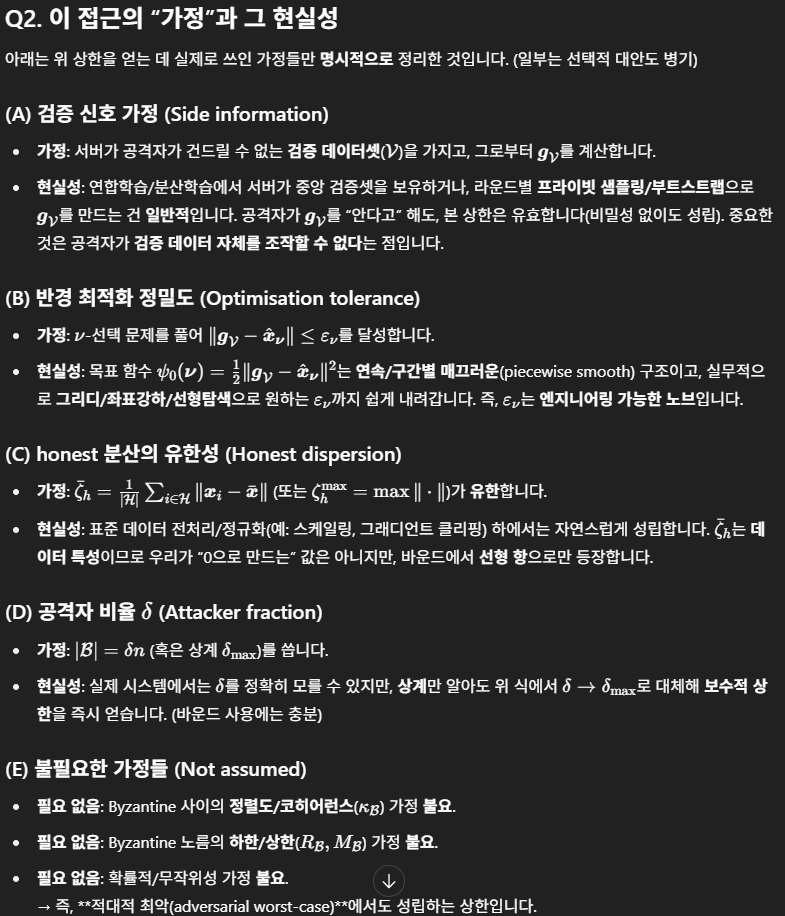
\includegraphics[
  width=0.75\paperwidth,
  height=\paperheight,
  keepaspectratio
]{figure/Worst-Case-02.png}
%
\noindent

\includegraphics[
  width=0.75\paperwidth,
  height=\paperheight,
  keepaspectratio
]{figure/Worst-Case-03.png}
\clearpage
\restoregeometry






































\clearpage
\appendix

\bigskip
\center\Huge{Graveyard}
\section*{Setup and Definitions}

\paragraph{Data.}
We have $n$ client vectors $\bm{x}_1,\dots,\bm{x}_n\in\mathbb{R}^d$, a center (initial point) $\bm{x}_0\in\mathbb{R}^d$, 
and a validation gradient (side information) $\bm{g}_{\mathcal{V}}\in\mathbb{R}^d$.
Let $\mathcal{H}$ be the index set of honest clients and $\mathcal{B}$ that of Byzantine clients; $\mathcal{H}\cup \mathcal{B}=\{1,\dots,n\}$ and $\mathcal{H}\cap \mathcal{B}=\emptyset$.

\paragraph{Directions and clipping ratios.}
For each $i$ with $\bm{x}_i\ne \bm{x}_0$ define the unit direction
\begin{equation}
\bm{d}_i \;:=\; \frac{\bm{x}_i-\bm{x}_0}{\|\bm{x}_i-\bm{x}_0\|}.
\label{eq:def-di}
\end{equation}
Given radii $\bm{\nu}=(\nu_1,\dots,\nu_n)\in \mathbb{R}^n$, the (client‑wise) centered clipping ratio is
\begin{equation}
\alpha_i(\bm{\nu}) \;:=\; \min\!\Bigl(1,\; \frac{\nu_i}{\|\bm{x}_i-\bm{x}_0\|}\Bigr)
\quad\in[0,1].
\label{eq:def-alpha}
\end{equation}

\paragraph{One-step aggregate.}
The clipped aggregate produced in a single step is
\begin{equation}
\hat {\bm{x}}_{\bm{\nu}} \;:=\; \bm{x}_0 \;+\; \frac{1}{n}\sum_{i=1}^n \alpha_i(\bm{\nu})\,\bigl(\bm{x}_i-\bm{x}_0\bigr).
\label{eq:def-xhat}
\end{equation}

\paragraph{Validation fitting objective.}
We choose $\bm{\nu}$ by minimizing the validation mismatch
\begin{equation}
\psi_0(\bm{\nu})\;:=\; \frac12 \,\bigl\|\bm{g}_{\mathcal{V}} - \hat {\bm{x}}_{\bm{\nu}}\bigr\|^2.
\label{eq:def-psi0}
\end{equation}

\bigskip

\section*{Step 1. Stationarity in $\bm{\nu_j}$}

Differentiate \eqref{eq:def-psi0} with respect to $\nu_j$.
By the chain rule,
\begin{equation}
\frac{\partial \psi_0}{\partial \nu_j}
= - \Bigl\langle \bm{g}_{\mathcal{V}}-\hat {\bm{x}}_{\bm{\nu}},\; \frac{\partial \hat {\bm{x}}_{\bm{\nu}}}{\partial \nu_j}\Bigr\rangle .
\label{eq:chain}
\end{equation}
From \eqref{eq:def-xhat} and \eqref{eq:def-alpha},
\[
\frac{\partial \hat {\bm{x}}_{\bm{\nu}}}{\partial \nu_j}
= \frac{1}{n}\,(\bm{x}_j-\bm{x}_0)\,\frac{\partial \alpha_j}{\partial \nu_j}
= \begin{cases}
\frac{1}{n}\,\bm{d}_j, & \text{if } \nu_j<\|\bm{x}_j-\bm{x}_0\| \quad(\text{unsaturated}),\\
0, & \text{if } \nu_j\ge \|\bm{x}_j-\bm{x}_0\|\quad(\text{saturated}).
\end{cases}
\]
Hence, at any (first‑order) stationary point with $\nu_j<\|\bm{x}_j-\bm{x}_0\|$,
\begin{equation}
\boxed{\;
\Bigl\langle \bm{g}_{\mathcal{V}}-\hat {\bm{x}}_{\bm{\nu}},\ \bm{d}_j\Bigr\rangle = 0.
\;}
\label{eq:stationarity}
\end{equation}

\bigskip

\section*{Step 2. Exact Projection Identity}

Introduce the error vector
\begin{equation}
\bm{e} \;:=\; \bm{g}_{\mathcal{V}} - \hat {\bm{x}}_{\bm{\nu}} .
\label{eq:def-e}
\end{equation}
Plugging \eqref{eq:def-xhat} into \eqref{eq:def-e} and taking inner product with $\bm{d}_j$,
\begin{align}
\langle \bm{e},\ \bm{d}_j\rangle
&= \Bigl\langle \bm{g}_{\mathcal{V}} - \bm{x}_0 - \frac{1}{n}\sum_{i=1}^n \alpha_i(\bm{\nu})\,(\bm{x}_i-\bm{x}_0),\ \bm{d}_j\Bigr\rangle
\nonumber\\
&= \underbrace{\langle \bm{g}_{\mathcal{V}} - \bm{x}_0,\ \bm{d}_j\rangle}_{\text{term (A)}}
\;-\; \frac{1}{n}\sum_{i=1}^n \alpha_i(\bm{\nu})\,\|\bm{x}_i-\bm{x}_0\|\ \langle \bm{d}_i,\ \bm{d}_j\rangle .
\label{eq:projection}
\end{align}
By \eqref{eq:stationarity}, the left‑hand side of \eqref{eq:projection} equals $0$ when $\nu_j$ is unsaturated.

\bigskip

\section*{Step 3. Splitting the Sum and Bounding Honest Cross Terms}

Split the sum in \eqref{eq:projection} over $\mathcal{H}$ and $\mathcal{B}$:
\begin{equation}
\sum_{i=1}^n \alpha_i\|\bm{x}_i-\bm{x}_0\|\langle \bm{d}_i,\bm{d}_j\rangle
\;=\;
\underbrace{\sum_{i\in \mathcal{H}} \alpha_i\|\bm{x}_i-\bm{x}_0\|\langle \bm{d}_i,\bm{d}_j\rangle}_{
  \colorbox{fluor}{%
    $\displaystyle
        S_{\mathcal{H}}(j)	
    $%
  }
}
\;+\;
\underbrace{\sum_{i\in \mathcal{B}} \alpha_i\|\bm{x}_i-\bm{x}_0\|\langle \bm{d}_i,\bm{d}_j\rangle}_{
  \colorbox{fluor}{%
    $\displaystyle
        S_{\mathcal{B}}(j)	
    $%
  }
} .
\label{eq:split}
\end{equation}

\paragraph{Assumptions for honest dispersion.}
Let $\bar{\bm{x}}:=\frac{1}{|\mathcal{H}|}\sum_{k\in \mathcal{H}} \bm{x}_k$ denote the honest mean.
Assume there exist finite constants
\begin{equation}
  \colorbox{fluor}{%
    $\displaystyle
        \|\bm{x}_0-\bar{\bm{x}}\|\le \varepsilon_0,
    $%
  }
\qquad
  \colorbox{fluor}{%
    $\displaystyle
        \|\bm{x}_i-\bar{\bm{x}}\|\le \zeta_h\quad \forall\, i\in \mathcal{H},
    $%
  }
\qquad
\|\bm{x}_i-\bm{x}_0\|\ge R_H>0\quad \forall\, i\in \mathcal{H}.
\label{eq:honest-assump}
\end{equation}
These say: the current center $\bm{x}_0$ and honest client vectors stay in a bounded neighborhood of the honest mean, and honest displacements are not degenerate.

\paragraph{Bounding a single honest inner product.}
Write $\bm{x}_i-\bm{x}_0=(\bar{\bm{x}}-\bm{x}_0)+(\bm{x}_i-\bar{\bm{x}})$.
Then
\begin{align}
|\langle \bm{d}_i,\bm{d}_j\rangle|
&= \frac{|\langle \bm{x}_i-\bm{x}_0,\ \bm{x}_j-\bm{x}_0\rangle|}{\|\bm{x}_i-\bm{x}_0\|\,\|\bm{x}_j-\bm{x}_0\|}
\nonumber\\
&= \frac{|\langle \bar{\bm{x}}-\bm{x}_0,\ \bm{x}_j-\bm{x}_0\rangle + \langle \bm{x}_i-\bar{\bm{x}},\ \bm{x}_j-\bm{x}_0\rangle|}{\|\bm{x}_i-\bm{x}_0\|\,\|\bm{x}_j-\bm{x}_0\|}
\nonumber\\
&\le \frac{\|\bar{\bm{x}}-\bm{x}_0\|\ \|\bm{x}_j-\bm{x}_0\| + \|\bm{x}_i-\bar{\bm{x}}\|\ \|\bm{x}_j-\bm{x}_0\|}{\|\bm{x}_i-\bm{x}_0\|\,\|\bm{x}_j-\bm{x}_0\|}
\le \frac{\varepsilon_0+\zeta_h}{\|\bm{x}_i-\bm{x}_0\|}
\le \frac{\varepsilon_0+\zeta_h}{R_H}.
\label{eq:single-honest-ip}
\end{align}

\paragraph{Bounding the honest sum \(S_{\mathcal{H}}(j)\).}
Using $0\le \alpha_i\le 1$ and \eqref{eq:single-honest-ip},
\begin{align}
|S_{\mathcal{H}}(j)|
&\le \sum_{i\in \mathcal{H}} \alpha_i\,\|\bm{x}_i-\bm{x}_0\|\ |\langle \bm{d}_i,\bm{d}_j\rangle|
\le \sum_{i\in \mathcal{H}} \|\bm{x}_i-\bm{x}_0\|\ \frac{\varepsilon_0+\zeta_h}{R_H}
\nonumber\\
&\le 
  \colorbox{fluor}{%
    $\displaystyle
        |\mathcal{H}|\, M_H \,\frac{\varepsilon_0+\zeta_h}{R_H}
        \;=:\; \rho_H,
    $%
  }
\label{eq:SH-bound}
\end{align}
where
$
  \colorbox{fluor}{%
    $\displaystyle
        M_H:=\max_{i\in \mathcal{H}}\|\bm{x}_i-\bm{x}_0\|
    $%
  }
$.

\bigskip

\section*{Step 4. Bounding Byzantine Cross Terms Except \(j\)}

Write $S_{\mathcal{B}}(j)=\alpha_j\|\bm{x}_j-\bm{x}_0\|\langle \bm{d}_j,\bm{d}_j\rangle + \sum_{i\in \mathcal{B},\,i\ne j}\alpha_i\|\bm{x}_i-\bm{x}_0\|\langle \bm{d}_i,\bm{d}_j\rangle$.
Since $\langle \bm{d}_j,\bm{d}_j\rangle=1$,
\begin{equation}
S_{\mathcal{B}}(j)=\alpha_j\|\bm{x}_j-\bm{x}_0\| + S_{\mathcal{B}}^{-j}(j),
\qquad
S_{\mathcal{B}}^{-j}(j):=\sum_{\substack{i\in \mathcal{B}\\ i\ne j}}\alpha_i\|\bm{x}_i-\bm{x}_0\|\langle \bm{d}_i,\bm{d}_j\rangle.
\label{eq:SB-split}
\end{equation}

\paragraph{Incoherence among Byzantine directions.}
Assume there exists $\kappa_{\mathcal{B}}\in[0,1)$ such that
\begin{equation}
  \colorbox{fluor}{%
    $\displaystyle
        |\langle \bm{d}_i,\bm{d}_j\rangle| \le \kappa_{\mathcal{B}}
            \qquad \text{for all distinct } i,j\in \mathcal{B}.
    $%
  }
\label{eq:byz-incoh}
\end{equation}
Let
$
  \colorbox{fluor}{%
    $\displaystyle
        M_{\mathcal{B}}:=\max_{i\in \mathcal{B}}\|\bm{x}_i-\bm{x}_0\|
    $%
  }
$ and define the maximal Byzantine clipping ratio
\begin{equation}
\alpha^{\max}_{\mathcal{B}} := \max_{i\in \mathcal{B}}\alpha_i.
\label{eq:alphamaxB}
\end{equation}
Then from \eqref{eq:SB-split} and \eqref{eq:byz-incoh},
\begin{equation}
|S_{\mathcal{B}}^{-j}(j)|
\le \sum_{\substack{i\in \mathcal{B}\\ i\ne j}} \alpha_i\,\|\bm{x}_i-\bm{x}_0\|\ |\langle \bm{d}_i,\bm{d}_j\rangle|
\le (|\mathcal{B}|-1)\,\alpha^{\max}_{\mathcal{B}}\, M_{\mathcal{B}}\,\kappa_{\mathcal{B}} .
\label{eq:SBminusj-bound}
\end{equation}

\bigskip

\section*{Step 5. Solving Stationarity for \(\alpha_j\) and a Fixed‑Point Bound}

Insert the split \eqref{eq:split} into \eqref{eq:projection}, use \eqref{eq:SH-bound}, \eqref{eq:SB-split}, \eqref{eq:SBminusj-bound}, and recall that $\langle \bm{e},\bm{d}_j\rangle=0$ by \eqref{eq:stationarity}.
We obtain
\begin{equation}
0
= \langle \bm{g}_{\mathcal{V}}-\bm{x}_0,\ \bm{d}_j\rangle
- \frac{1}{n}\Bigl( \alpha_j\|\bm{x}_j-\bm{x}_0\| + S_{\mathcal{B}}^{-j}(j) + S_{\mathcal{H}}(j) \Bigr).
\label{eq:stationarity-expanded}
\end{equation}
Rearranging \eqref{eq:stationarity-expanded} yields the exact identity
\begin{equation}
\alpha_j
= \frac{ n\,\langle \bm{g}_{\mathcal{V}}-\bm{x}_0,\ \bm{d}_j\rangle - S_{\mathcal{B}}^{-j}(j) - S_{\mathcal{H}}(j)}{\|\bm{x}_j-\bm{x}_0\|}.
\label{eq:alpha-exact}
\end{equation}
Taking absolute values and using \eqref{eq:SH-bound} and \eqref{eq:SBminusj-bound},
\begin{equation}
|\alpha_j|
\;\le\;
\frac{ n\,|\langle \bm{g}_{\mathcal{V}}-\bm{x}_0,\ \bm{d}_j\rangle|}{\|\bm{x}_j-\bm{x}_0\|}
\;+\;
\frac{ \rho_H }{\|\bm{x}_j-\bm{x}_0\|}
\;+\;
\frac{ (|\mathcal{B}|-1)\,M_{\mathcal{B}}\,\kappa_{\mathcal{B}} }{\|\bm{x}_j-\bm{x}_0\|}\ \alpha^{\max}_{\mathcal{B}} .
\label{eq:alpha-ineq}
\end{equation}
Let
$
  \colorbox{fluor}{%
    $\displaystyle
        R_{\mathcal{B}}:=\min_{i\in \mathcal{B}}\|\bm{x}_i-\bm{x}_0\|
    $%
  }
$
and
\begin{equation}
  \colorbox{fluor}{%
    $\displaystyle
        \eta := \max_{j\in \mathcal{B}} |\langle \bm{g}_{\mathcal{V}}-\bm{x}_0,\ \bm{d}_j\rangle|.
    $%
  }
\label{eq:eta-def}
\end{equation}
Then from \eqref{eq:alpha-ineq},
\begin{equation}
\max_{j\in \mathcal{B}} |\alpha_j|
\;\le\;
\underbrace{\frac{n\,\eta + \rho_H}{R_{\mathcal{B}}}}_{=:~\tau}
\;+\;
  \colorbox{fluor}{%
    $\displaystyle
\underbrace{\frac{(|\mathcal{B}|-1)\,\kappa_{\mathcal{B}}}{R_{\mathcal{B}}}\  M_{\mathcal{B}}}_{=:~\beta}
    $%
  }\  \alpha^{\max}_{\mathcal{B}} .
\label{eq:alpha-fp}
\end{equation}
Since the left side equals $\alpha^{\max}_{\mathcal{B}}$ by definition \eqref{eq:alphamaxB}, \eqref{eq:alpha-fp} is a \emph{fixed‑point inequality}:
\begin{equation}
\alpha^{\max}_{\mathcal{B}} \;\le\; \tau + \beta\,\alpha^{\max}_{\mathcal{B}} .
\label{eq:fp-short}
\end{equation}
If the incoherence factor satisfies 
$
  \colorbox{alert}{%
    $\displaystyle
        \beta<1	
    $%
  }
$
(i.e., 
$
  \colorbox{alert}{%
    $\displaystyle
        R_{\mathcal{B}}>(|\mathcal{B}|-1)M_{\mathcal{B}}\kappa_{\mathcal{B}}	
    $%
  }
$),
then \eqref{eq:fp-short} implies the explicit bound
\begin{equation}
\boxed{\;
\alpha^{\max}_{\mathcal{B}} \;\le\; \frac{\tau}{1-\beta}
\;=\;
\frac{n\,\eta + \rho_H}{R_{\mathcal{B}} - (|\mathcal{B}|-1)M_{\mathcal{B}}\kappa_{\mathcal{B}}}.
\;}
\label{eq:alphamax-final}
\end{equation}



\bigskip
\paragraph{Interpretation.}
The quantity $\eta$ in \eqref{eq:eta-def} measures how well the validation direction $\bm{g}_{\mathcal{V}}$ suppresses any Byzantine direction $\bm{d}_j$ via the inner product; 
$\rho_H$ from \eqref{eq:SH-bound} is the (controlled) leakage from honest cross terms; 
$\beta$ captures mutual alignment among Byzantine directions.
When $\eta$ and $\rho_H$ are small (strong validation hint, tight honest dispersion) and $\beta<1$ (no near‑collinearity among Byzantine directions), \eqref{eq:alphamax-final} forces every Byzantine clipping ratio to be small.
\begin{align*}
%
\eta
    &:= \max_{j\in \mathcal{B}} |\langle \bm{g}_{\mathcal{V}}-\bm{x}_0,\ \bm{d}_j\rangle|.\\
%
\rho_H
    &:= |\mathcal{H}|\, M_H \,\frac{\varepsilon_0+\zeta_h}{R_H},\\
%
M_H
    &:= \max_{i\in \mathcal{H}}\|\bm{x}_i-\bm{x}_0\|,\\
%
\varepsilon_0
    &:= \|\bm{x}_0-\bar{\bm{x}}\|\\
%
\zeta_h
    &:=
    \max_{i \in \mathcal{H}}
        \|\bm{x}_i-\bar{\bm{x}}\|,\\
%
\beta
    &:= \frac{(|\mathcal{B}|-1)\,\kappa_{\mathcal{B}}}{R_{\mathcal{B}}}\  M_{\mathcal{B}},\\
%
  \colorbox{fluor}{%
    $\displaystyle
    \kappa_{\mathcal{B}}
    $%
  }
    &:= \max_{
        \substack{
            i \neq j,\\
            i,j \in \mathcal{B}
        }
    } |\langle \bm{d}_i,\bm{d}_j\rangle|,\\
%
  \colorbox{fluor}{%
    $\displaystyle
    R_{\mathcal{B}}	
    $%
  }
    &:=\min_{j\in \mathcal{B}}\|\bm{x}_j-\bm{x}_0\|,\\
%
  \colorbox{fluor}{%
    $\displaystyle
    M_{\mathcal{B}}	
    $%
  }
    &:= \max_{j\in \mathcal{B}}\|\bm{x}_j-\bm{x}_0\|.
%
\end{align*}
Three values at the bottom are under full control of omniscient Byzantines.


\bigskip
\section*{Step 6. Consequence for the One‑Step Aggregate}

From \eqref{eq:def-xhat},
\begin{align}
\hat {\bm{x}}_{\bm{\nu}}
&= \bm{x}_0 + \frac{1}{n}\sum_{i\in \mathcal{H}} \alpha_i(\bm{\nu})(\bm{x}_i-\bm{x}_0)
     + \frac{1}{n}\sum_{j\in \mathcal{B}} \alpha_j(\bm{\nu})(\bm{x}_j-\bm{x}_0).
\label{eq:xhat-split}
\end{align}
Hence the Byzantine contribution is bounded by
\begin{equation}
\Bigl\| \frac{1}{n}\sum_{j\in \mathcal{B}} \alpha_j(\bm{\nu})(\bm{x}_j-\bm{x}_0) \Bigr\|
\;\le\;
\frac{|\mathcal{B}|}{n}\ \alpha^{\max}_{\mathcal{B}}\, M_{\mathcal{B}}
\;=\;
\delta\ \alpha^{\max}_{\mathcal{B}}\, M_{\mathcal{B}},
\label{eq:byz-contrib}
\end{equation}
where $\delta=|\mathcal{B}|/n$.
Combining \eqref{eq:byz-contrib} with \eqref{eq:alphamax-final} gives a fully explicit upper bound on the Byzantine distortion of the one‑step aggregate in terms of \emph{observable or design} constants 
$(\varepsilon_0,\zeta_h,R_H)$,
$(M_{\mathcal{B}},R_{\mathcal{B}},\kappa_{\mathcal{B}})$,
and the validation alignment $\eta$.



\clearpage
% ============================================================
% Section: Byzantine Contribution Bound Without Using \beta
% (drop-in, notation aligned with \bm{} vectors and \mathcal{} sets)
% ============================================================
\section{Byzantine Contribution Bound Without Using \texorpdfstring{$\beta$}{beta}}
\label{sec:byz-no-beta}

This section provides a bound on the \emph{actual Byzantine contribution} that
does not depend on the norm parameters
$R_{\mathcal{B}}=\min_{j\in\mathcal{B}}\|\bm{x}_j-\bm{x}_0\|$ and
$M_{\mathcal{B}}=\max_{j\in\mathcal{B}}\|\bm{x}_j-\bm{x}_0\|$.
The bound is stated directly in terms of: (i) the \emph{directional coherence}
among Byzantine directions, (ii) the \emph{validation alignment} with Byzantine
directions, and (iii) an a priori bound on the honest cross term.

\paragraph{Notation and standing assumptions.}
Let $\mathcal{H}$ and $\mathcal{B}$ denote the honest and Byzantine index sets,
respectively, with $|\mathcal{B}|=\delta n$.
At the current round, the center is $\bm{x}_0\in\mathbb{R}^d$ and the client
proposals are $\bm{x}_i\in\mathbb{R}^d$.
Define unit directions
\begin{equation}
\bm{d}_i \;:=\; \frac{\bm{x}_i-\bm{x}_0}{\|\bm{x}_i-\bm{x}_0\|}
\quad (\,\bm{x}_i\neq \bm{x}_0\,),
\qquad
\alpha_i(\bm{\nu}) \;:=\; \min\!\Bigl(1,\;\frac{\nu_i}{\|\bm{x}_i-\bm{x}_0\|}\Bigr)\in[0,1].
\label{eq:sec-nobeta-defs}
\end{equation}
The one-step clipped aggregate is
$\hat{\bm{x}}_{\bm{\nu}}
= \bm{x}_0 + \frac{1}{n}\sum_{i=1}^n \alpha_i(\bm{\nu})(\bm{x}_i-\bm{x}_0)$.
As in the main text, we assume the \emph{stationarity} condition holds for every
\emph{unsaturated} coordinate (i.e.\ $\nu_j<\|\bm{x}_j-\bm{x}_0\|$):
\begin{equation}
\bigl\langle \bm{g}_{\mathcal{V}}-\hat{\bm{x}}_{\bm{\nu}},\ \bm{d}_j\bigr\rangle \;=\; 0.
\label{eq:sec-nobeta-stationarity}
\end{equation}
We will only invoke \eqref{eq:sec-nobeta-stationarity} for indices 
$
  \colorbox{fluor}{%
    $\displaystyle
        j\in\mathcal{B}	
    ~\textnormal{that are unsaturated.}
    $%
  }
$
\footnote{If a particular $j\in\mathcal{B}$ is saturated, then $\alpha_j=1$ and the bound below trivially controls its contribution through the $\kappa_{\mathcal{B}}$ term; alternatively, one can work with subgradient KKT conditions.}

Finally, define:
\begin{equation}
\eta \;:=\; \max_{j\in\mathcal{B}}\ \bigl|\langle \bm{g}_{\mathcal{V}}-\bm{x}_0,\ \bm{d}_j\rangle\bigr|,
\qquad
\kappa_{\mathcal{B}} \;:=\; \max_{\substack{i,j\in\mathcal{B}\\ i\neq j}}
\bigl|\langle \bm{d}_i,\bm{d}_j\rangle\bigr|,
\label{eq:sec-nobeta-eta-kappa}
\end{equation}
and let $\rho_H$ be any (uniform-in-$j$) bound on the honest cross term
\begin{equation}
\Bigl|\,S_{\mathcal{H}}(j)\Bigr|
\;:=\;
\Biggl|\,
\sum_{i\in\mathcal{H}}
\alpha_i(\bm{\nu})\ \|\bm{x}_i-\bm{x}_0\|\ \langle \bm{d}_i,
  \colorbox{fluor}{%
    $\displaystyle
        \bm{d}_j	
    $%
  }
\rangle
\,\Biggr|
\ \le\
\rho_H,
\qquad
  \colorbox{fluor}{%
    $\displaystyle
        \forall\,j\in\mathcal{B}.	
    $%
  }
\label{eq:sec-nobeta-rhoH}
\end{equation}
(For example, one may take the explicit $\rho_H$ from the honest-dispersion bound in the main text.)

We now work with the \emph{Byzantine contribution magnitudes}
\begin{equation}
C_j \;:=\; \alpha_j(\bm{\nu})\ \|\bm{x}_j-\bm{x}_0\|,
\qquad
C_{\max} \;:=\; \max_{j\in\mathcal{B}} C_j .
\label{eq:sec-nobeta-Cdefs}
\end{equation}

\begin{lemma}[Projection identity for a fixed Byzantine index]
\label{lem:nobeta-proj}
Fix $j\in\mathcal{B}$ such that $\nu_j<\|\bm{x}_j-\bm{x}_0\|$.
Then, using \eqref{eq:sec-nobeta-stationarity},
\begin{equation}
n\ \bigl\langle \bm{g}_{\mathcal{V}}-\bm{x}_0,\ \bm{d}_j\bigr\rangle
\;=\;
\underbrace{\sum_{i\in\mathcal{H}}\alpha_i\|\bm{x}_i-\bm{x}_0\|\,\langle \bm{d}_i,\bm{d}_j\rangle}_{S_{\mathcal{H}}(j)}
\;+\;
\underbrace{\sum_{i\in\mathcal{B}}\alpha_i\|\bm{x}_i-\bm{x}_0\|\,\langle \bm{d}_i,\bm{d}_j\rangle}_{S_{\mathcal{B}}(j)}.
\label{eq:nobeta-proj-identity}
\end{equation}
Moreover,
\begin{equation}
S_{\mathcal{B}}(j) \;=\; C_j \;+\;
\sum_{\substack{i\in\mathcal{B}\\ i\neq j}}
C_i\,\langle \bm{d}_i,\bm{d}_j\rangle .
\label{eq:nobeta-SB-decomp}
\end{equation}
\end{lemma}

\begin{proof}
From $\hat{\bm{x}}_{\bm{\nu}}=\bm{x}_0+\frac1n\sum_i \alpha_i(\bm{\nu})(\bm{x}_i-\bm{x}_0)$ and
\eqref{eq:sec-nobeta-stationarity}, we get
\[
0=\bigl\langle \bm{g}_{\mathcal{V}}-\hat{\bm{x}}_{\bm{\nu}},\bm{d}_j\bigr\rangle
=\bigl\langle \bm{g}_{\mathcal{V}}-\bm{x}_0,\bm{d}_j\bigr\rangle
-\frac1n \sum_{i=1}^n \alpha_i\|\bm{x}_i-\bm{x}_0\|\langle \bm{d}_i,\bm{d}_j\rangle,
\]
which rearranges to \eqref{eq:nobeta-proj-identity}. The decomposition
\eqref{eq:nobeta-SB-decomp} is the definition of $C_i$ plus separating the $i=j$ term.
\end{proof}

\begin{theorem}[Byzantine magnitude bound independent of norms]
\label{thm:nobeta-Cmax}
Assume \eqref{eq:sec-nobeta-rhoH} holds and define $\eta,\kappa_{\mathcal{B}}$ as in
\eqref{eq:sec-nobeta-eta-kappa}. Then
\begin{equation}
\bigl(1-(|\mathcal{B}|-1)\,\kappa_{\mathcal{B}}\bigr)\ C_{\max}
\;\le\;
n\,\eta + \rho_H.
\label{eq:nobeta-Cmax-core}
\end{equation}
In particular, if 
$
  \colorbox{alert}{%
    $\displaystyle
        (|\mathcal{B}|-1)\,\kappa_{\mathcal{B}}<1
    $%
  }
$, then
\begin{equation}
\boxed{\;
C_{\max}
\;\le\;
\frac{n\,\eta + \rho_H}{\,1-(|\mathcal{B}|-1)\,\kappa_{\mathcal{B}}\,}.
\;}
\label{eq:nobeta-Cmax}
\end{equation}
\end{theorem}

\begin{proof}
Fix $j\in\mathcal{B}$ unsaturated and start from \eqref{eq:nobeta-proj-identity}.
Taking absolute values and using \eqref{eq:sec-nobeta-eta-kappa} and \eqref{eq:sec-nobeta-rhoH},
\[
C_j
\;\le\;
n\,\eta \;+\; |S_{\mathcal{H}}(j)|
\;+\;\sum_{\substack{i\in\mathcal{B}\\ i\neq j}} C_i\,|\langle \bm{d}_i,\bm{d}_j\rangle|
\;\le\;
n\,\eta \;+\; \rho_H \;+\; (|\mathcal{B}|-1)\,\kappa_{\mathcal{B}}\ C_{\max}.
\]
Now take the maximum over $j\in\mathcal{B}$ on the left to obtain
\[
C_{\max}
\;\le\;
n\,\eta \;+\; \rho_H \;+\; (|\mathcal{B}|-1)\,\kappa_{\mathcal{B}}\ C_{\max},
\]
which rearranges to \eqref{eq:nobeta-Cmax-core} and yields \eqref{eq:nobeta-Cmax}
when $(|\mathcal{B}|-1)\kappa_{\mathcal{B}}<1$.
\end{proof}

\begin{corollary}[Aggregate Byzantine contribution]
\label{cor:nobeta-agg}
The total Byzantine contribution to the one-step aggregate satisfies
\begin{equation}
\Biggl\|
\frac{1}{n}\sum_{j\in\mathcal{B}} \alpha_j(\bm{\nu})\,(\bm{x}_j-\bm{x}_0)
\Biggr\|
\ \le\
\frac{|\mathcal{B}|}{n}\,C_{\max}
\ =\
\delta\,C_{\max}
\ \le\
\boxed{\;
\frac{\delta}{\,1-(|\mathcal{B}|-1)\,\kappa_{\mathcal{B}}\,}\ \bigl(n\,\eta+\rho_H\bigr).
\;}
\label{eq:nobeta-agg}
\end{equation}
\end{corollary}

\paragraph{Remarks.}
(i) The bounds \eqref{eq:nobeta-Cmax}–\eqref{eq:nobeta-agg} do \emph{not} involve
$R_{\mathcal{B}}$ or $M_{\mathcal{B}}$; hence they are robust even if an attacker
knows $\bm{x}_0$ and attempts to manipulate vector norms.
(ii) The only structural requirement is $(|\mathcal{B}|-1)\kappa_{\mathcal{B}}<1$,
i.e.\ Byzantine directions are not nearly collinear; this condition is typically
mild in moderate/high dimension (and can be enforced with tiny dithering).
(iii) The \emph{numerators} $n\eta+\rho_H$ are \emph{algorithmically controllable}:
validation fitting and iteration can drive $\eta\!\downarrow\!0$, and the honest
bias/dispersion bound $\rho_H$ can be reduced by iteration and data curation.
Consequently, \eqref{eq:nobeta-agg} shows the Byzantine impact can be made
arbitrarily small under a mild directional incoherence condition.

\section*{Sufficient Conditions for \texorpdfstring{$\beta<1$}{beta<1}}

To make this supplement self-contained and directly pluggable into \texttt{res.tex}, we recall the key quantities and the bound we reference. Let $\cH$ and $\cB$ be the honest and Byzantine index sets, respectively. For each client $i$, let $\vx_i\in\R^{d}$ and let the iteration center be $\vx_{0}\in\R^{d}$. Define directions $\vd_i := (\vx_i-\vx_0)/\|\vx_i-\vx_0\|$ whenever $\vx_i\neq \vx_0$. Let
\[
M_{\cB}:=\max_{i\in \cB}\|\vx_i-\vx_0\|,
\quad
R_{\cB}:=\min_{i\in \cB}\|\vx_i-\vx_0\|,
\quad
\kappa_{\cB}:=\max_{\substack{i,j\in \cB\\ i\neq j}}|\langle \vd_i,\vd_j\rangle|.
\]
Write $\alpha^{\max}_{\cB}:=\max_{i\in \cB}\alpha_i$ for the maximal Byzantine clipping ratio, and
\[
\eta := \max_{j\in \cB}|\langle \vg_{\cV}-\vx_0,\ \vd_j\rangle|,
\qquad
\rho_{H}:=|\cH|\,M_{H}\,(\varepsilon_{0}+\zeta_{h})/R_{H},
\]
where $(\varepsilon_{0},\zeta_{h},R_{H},M_{H})$ summarize the honest dispersion/bias constants defined in the main text.

The fixed-point inequality derived earlier yields the explicit bound
\begin{equation}
\boxed{\;
\alpha^{\max}_{\cB}
\ \le\
\frac{n\,\eta+\rho_H}{\;R_{\cB} - (|\cB|-1)\,M_{\cB}\,\kappa_{\cB}\;}
\quad\text{whenever}\quad
R_{\cB} > (|\cB|-1)\,M_{\cB}\,\kappa_{\cB}.
\;}
\label{eq:alphamax-final}
\end{equation}
We now state clean sufficient conditions ensuring the denominator in \eqref{eq:alphamax-final} is positive, i.e., $\beta<1$ below.

\section*{Sufficient Conditions for \texorpdfstring{$\beta<1$}{beta<1}}

Recall (from \eqref{eq:alphamax-final}) that
\[
\beta \;=\; \frac{(|\cB|-1)\,M_{\cB}\,\kappa_{\cB}}{R_{\cB}},
\qquad
M_{\cB}:=\max_{i\in \cB}\|\vx_i-\vx_0\|,
\ \ R_{\cB}:=\min_{i\in \cB}\|\vx_i-\vx_0\|,
\ \ \kappa_{\cB}:=\max_{\substack{i,j\in \cB\\ i\neq j}}|\langle \vd_i,\vd_j\rangle|.
\]

\begin{lemma}[Equivalences]
\label{lem:beta-equiv}
The following are equivalent:
\begin{align*}
\text{\em(i)}\quad& \beta<1,\\
\text{\em(ii)}\quad& R_{\cB} > (|\cB|-1)\,M_{\cB}\,\kappa_{\cB},\\
\text{\em(iii)}\quad& \kappa_{\cB} < \frac{R_{\cB}}{(|\cB|-1)\,M_{\cB}},\\
\text{\em(iv)}\quad& |\cB|-1 < \frac{R_{\cB}}{M_{\cB}\,\kappa_{\cB}}\quad(\text{when }\kappa_{\cB}>0).
\end{align*}
\emph{Proof.} All statements are immediate rearrangements of
$\beta = (|\cB|-1)M_{\cB}\kappa_{\cB}/R_{\cB}$.
\hfill\(\square\)
\end{lemma}

\begin{corollary}[Equal Byzantine magnitudes]
\label{cor:equal-norms}
If all Byzantine displacements have the same norm
$\|\vx_i-\vx_0\|\equiv r_{\cB}$ (thus $R_{\cB}=M_{\cB}=r_{\cB}$), then
\[
\beta \;=\; (|\cB|-1)\,\kappa_{\cB}
\quad\text{and hence}\quad
\beta<1 \iff \kappa_{\cB} < \frac{1}{|\cB|-1}.
\]
\end{corollary}

\begin{corollary}[Bound on attacker count for given geometry]
\label{cor:count}
Suppose $\kappa_{\cB}\le \bar\kappa<1$ and $R_{\cB}\ge r>0$, $M_{\cB}\le m<\infty$.
If
\[
|\cB| \;\le\; 1 + \Big\lfloor \frac{r}{m\,\bar\kappa}\Big\rfloor,
\]
then $\beta<1$.
\emph{Proof.} By Lemma~\ref{lem:beta-equiv}(iv),
$|\cB|-1 < R_{\cB}/(M_{\cB}\kappa_{\cB})\ge r/(m\bar\kappa)$.
\hfill\(\square\)
\end{corollary}

\begin{corollary}[Angular separation]
\label{cor:angle}
Let $\theta_{\min}$ be the minimal pairwise angle between Byzantine directions:
\[
\theta_{\min} \;:=\; \min_{\substack{i,j\in \cB\\ i\neq j}}
\arccos\bigl(|\langle \vd_i,\vd_j\rangle|\bigr).
\]
Then $\kappa_{\cB}=\max_{i\neq j}|\langle \vd_i,\vd_j\rangle|\le \cos\theta_{\min}$, and a sufficient condition for $\beta<1$ is
\[
\theta_{\min} \;>\;
\arccos\!\Bigl(\frac{R_{\cB}}{(|\cB|-1)\,M_{\cB}}\Bigr).
\]
In particular, if Byzantine directions are pairwise orthogonal
($\theta_{\min}=90^\circ$, so $\kappa_{\cB}=0$), then $\beta=0$ automatically.
\end{corollary}

\begin{corollary}[Norm separation]
\label{cor:norm-sep}
If Byzantine norms are not too imbalanced, i.e.,
$R_{\cB}/M_{\cB} \ge \gamma$ for some $\gamma\in(0,1]$, and the pairwise coherence satisfies $\kappa_{\cB}\le c$, then
\[
\beta \;\le\; \frac{|\cB|-1}{\gamma}\,c.
\]
Hence a simple sufficient condition is
\[
c \;<\; \frac{\gamma}{|\cB|-1}
\quad\text{(equivalently, }\kappa_{\cB} < \gamma/(|\cB|-1)\text{)}.
\]
\end{corollary}

\paragraph{Practical reading.}
\begin{itemize}
\item \textbf{Few attackers or weak alignment.} For fixed geometry $(R_{\cB},M_{\cB})$,
either keep $|\cB|$ small or ensure Byzantine directions are poorly aligned ($\kappa_{\cB}$ small).
\item \textbf{Equal‑norm case is sharp.} When $R_{\cB}=M_{\cB}$, the clean threshold is
$\kappa_{\cB}<1/(|\cB|-1)$ (Cor.~\ref{cor:equal-norms}).
\item \textbf{Angle or coherence budgets.}
If you can certify a minimum inter‑attacker angle $\theta_{\min}$,
then Cor.~\ref{cor:angle} turns it into a direct check.
\item \textbf{Robust to scaling.}
If attackers cannot make one vector arbitrarily small ($R_{\cB}$ not tiny)
while growing the others ($M_{\cB}$ not huge), Cor.~\ref{cor:norm-sep} gives an immediate margin.
\end{itemize}

\paragraph{Example: High–dimensional random directions (``extremely mild'' coherence).}
Let $m:=|\cB|$ and suppose the Byzantine directions $\{\vd_i\}_{i\in \cB}$ are independent and uniformly
distributed on the unit sphere $\mathbb{S}^{d-1}$ (or sufficiently “random‑looking” so that spherical
concentration applies).

\medskip
\noindent\textbf{Lemma (Spherical concentration + union bound).}
For any $t\in(0,1)$,
\[
\mathbb{P}\!\left(\max_{i\neq j\in \cB}|\langle \vd_i,\vd_j\rangle|\;\ge\;t\right)
\;\le\; 2\,m(m-1)\,\exp\!\Bigl(-\tfrac{(d-1)\,t^{2}}{2}\Bigr).
\]
\emph{Sketch.} For fixed $i\neq j$, $|\langle \vd_i,\vd_j\rangle|$ is sub‑Gaussian with tail
$\le 2\exp(-(d-1)t^2/2)$; take a union bound over $m(m-1)$ pairs.

\medskip
\noindent\textbf{Dimension threshold for the norm–separation condition.}
Target the sufficient condition of Cor.~\ref{cor:norm-sep} with $c=t=\gamma/(m-1)$.
Given failure probability $\delta\in(0,1)$, it suffices to pick
\begin{equation}
d \;\ge\; 1 \;+\; \frac{2\,(m-1)^{2}}{\gamma^{2}}\,
\log\!\Bigl(\frac{2\,m(m-1)}{\delta}\Bigr)
\label{eq:d-threshold}
\end{equation}
so that with probability at least $1-\delta$ one has
\(
\kappa_{\cB}=\max_{i\neq j}|\langle \vd_i,\vd_j\rangle|
\le \gamma/(m-1)
\)
and hence
\(
\beta \le \frac{m-1}{\gamma}\,\kappa_{\cB}<1
\)
by Cor.~\ref{cor:norm-sep}.

\medskip
\noindent\textbf{Numerical illustrations.}
\begin{itemize}
\item \emph{Moderate $d$, few attackers.}  
Take $\gamma=1$ (equal Byzantine norms), $m=5$ (four attackers), and $\delta=0.01$.  
Then \eqref{eq:d-threshold} gives
\[
d \;\ge\; 1 + 2\cdot 4^{2}\,\log\!\Bigl(\tfrac{2\cdot 5\cdot 4}{0.01}\Bigr)
\;=\; 1 + 32\,\log(4000)
\;\approx\; 267.
\]
Thus in dimension $d\!\ge\!267$, with probability at least $99\%$ we have
\(\kappa_{\cB} \le 1/4\) and the condition \(\beta<1\) holds.
\item \emph{Larger $m$, still mild in high $d$.}  
Let $\gamma=1$, $m=8$ and $\delta=10^{-6}$.  
Then \eqref{eq:d-threshold} yields
\[
d \;\ge\; 1 + 2\cdot 7^{2}\,\log\!\Bigl(\tfrac{2\cdot 8\cdot 7}{10^{-6}}\Bigr)
\;\approx\; 1 + 98\cdot 18.53
\;\approx\; 1818.
\]
So in $d\!\ge\!1818$ (well within common model dimensions), with probability at least $1-10^{-6}$
we have \(\kappa_{\cB} \le 1/7\) and hence \(\beta<1\).
\end{itemize}

\medskip
\noindent\textbf{Two–attacker special case (equal norms).}
When $m=2$ and $R_{\cB}=M_{\cB}$ (equal norms), the condition is simply \(\kappa_{\cB}<1\),
i.e., the two directions are not perfectly collinear. This holds with probability~$1$ under any
continuous‑noise model and is thus \emph{extremely mild}. For a robust quantitative margin, one may
enforce $\kappa_{\cB}\le 1-\xi$ ($\xi\in(0,1)$), which yields the well‑conditioned bound
\(
\alpha_{\cB}^{\max}\le (n\,\eta+\rho_H)/(R_{\cB}\,\xi)
\)
from the fixed‑point inequality.













\end{document}
